% From this directory, run pdflatex -halt-on-error manual.tex twice.
% The resulting manual.pdf is distributed as ../../SensCalc_manual.pdf.
\documentclass[11pt,a4paper]{article}
\usepackage[T1]{fontenc}
\usepackage[utf8]{inputenc}
\usepackage{lmodern}
\usepackage[margin=24mm,headheight=15pt]{geometry}
\usepackage{microtype,amsmath,amssymb,booktabs,tabularx,array,longtable}
\usepackage{enumitem,fvextra,xcolor,tikz,fancyhdr,needspace}
\usetikzlibrary{arrows.meta,positioning}
\definecolor{linkblue}{HTML}{185A8A}
\definecolor{lightblue}{HTML}{EFF5F9}
\usepackage[unicode,colorlinks=true,linkcolor=linkblue,urlcolor=linkblue,citecolor=linkblue,
  pdftitle={SensCalc: user guide},pdfauthor={Maksym Ovchynnikov},
  pdfsubject={Physics models, calculations and use of SensCalc}]{hyperref}
\usepackage{bookmark}
\setlength{\parindent}{0pt}
\setlength{\parskip}{5pt plus 1pt}
\setlength{\emergencystretch}{2em}
\widowpenalty=10000
\clubpenalty=10000
\renewcommand{\arraystretch}{1.22}
\newcolumntype{Y}{>{\raggedright\arraybackslash}X}
\newcolumntype{P}[1]{>{\raggedright\arraybackslash}p{#1}}
\setlist{nosep,leftmargin=1.5em,topsep=5pt}
\setcounter{tocdepth}{1}
\pagestyle{fancy}
\fancyhf{}
\fancyhead[L]{\small\textsc{SensCalc}}
\fancyhead[R]{\small User guide}
\fancyfoot[C]{\small\thepage}
\renewcommand{\headrulewidth}{0.3pt}
\newcommand{\code}[1]{\texttt{\detokenize{#1}}}
\newcommand{\arxiv}[1]{\href{https://arxiv.org/abs/#1}{arXiv:#1}}
\newcommand{\GeV}{\mathrm{GeV}}
\newcommand{\Br}{\operatorname{Br}}
\newcommand{\hc}{\mathrm{h.c.}}
\newcommand{\dd}{\mathrm{d}}
\DefineVerbatimEnvironment{Code}{Verbatim}{fontsize=\small,breaklines=true,breakanywhere=true,
  frame=single,rulecolor=\color{black!20},framesep=6pt}
\begin{document}
\begin{center}
  {\LARGE\bfseries SensCalc: user guide}\par
  \vspace{5pt}
  {\large Maksym Ovchynnikov}\par
  \href{mailto:o.maxim@gmail.com}{o.maxim@gmail.com}\par
  November 2026
\end{center}

SensCalc is a \href{https://www.wolfram.com/mathematica/}{Wolfram Mathematica} package for calculating expected signals from long-lived particles (LLPs) and the sensitivity of accelerator experiments. It combines production spectra, decay probabilities, detector geometry and selection cuts. The calculation method and model phenomenology are described in the works collected in Section~\ref{sec:references}.

Production and detection are tabulated separately, allowing experiments to be compared using common physical inputs. The event generator returns weighted LLP decays for further detector studies. This guide explains the physics conventions, the notebook workflow, and the meaning of the saved results.

\href{https://github.com/maksymovchynnikov/SensCalc}{Repository and online documentation}
\hfill
\href{https://github.com/maksymovchynnikov/SensCalc/issues}{Questions and bug reports}

\tableofcontents
\clearpage

\section{Calculation method}\label{sec:method}
\subsection{Expected number of decays}
For a search that detects the decay of one LLP, SensCalc evaluates
\begin{equation}\label{eq:yield}
 N_{\mathrm{events}}=\sum_i N_i\int \dd\theta\,\dd E\,\dd z\,
 f_i(\theta,E)\,\epsilon_{\mathrm{az}}(\theta,z)\,
 \frac{\dd P_{\mathrm{decay}}}{\dd z}\,
 \Br_{\mathrm{vis}}\,\epsilon_{\mathrm{dec}}(m,\theta,E,z).
\end{equation}
Here $i$ labels a production mechanism, $N_i$ is the total number of LLPs produced through it, and $f_i$ is their normalized distribution in polar angle $\theta$ and energy $E$. The LLP mass is $m$, and $z$ measures longitudinal displacement from the production point. Angles are in radians, energies and masses in GeV, and distances in metres.

The fraction $\epsilon_{\mathrm{az}}$ averages over the azimuthal angle: at fixed $(\theta,z)$ it measures which positions lie inside the decay volume. The factor $\Br_{\mathrm{vis}}$ is the sum of branching fractions for the selected decay channels. Conditional on those channels and an allowed vertex, $\epsilon_{\mathrm{dec}}$ is the fraction of decays that pass the detector requirements. These factors describe distinct parts of the signal probability.

For a particle travelling toward positive $z$, its mean longitudinal decay length is
\begin{equation}\label{eq:lifetime}
 \lambda_z=c\tau\frac{\sqrt{E^2-m^2}}{m}\cos\theta,
 \qquad
 \frac{\dd P_{\mathrm{decay}}}{\dd z}=\frac{e^{-z/\lambda_z}}{\lambda_z},
\end{equation}
where $c\tau$ is the proper decay length. The probability of a decay between $z_1$ and $z_2$ along an allowed ray is $e^{-z_1/\lambda_z}-e^{-z_2/\lambda_z}$. Geometry determines these intervals; the boosted lifetime controls the competition between reaching the detector and escaping it.

For fixed-target production, $N_i$ contains the exposure, the parent yield per incident particle, branching fractions and LLP multiplicity. Collider calculations use the integrated luminosity and relevant cross sections. The facility definitions account for charge-conjugate parent populations and, for symmetric colliders, the two hemispheres. The production density uses the measure $\dd\theta\,\dd E$, including when the tabulation nodes are logarithmically spaced.

\subsection{Reusable inputs}
The four main notebooks divide the calculation into the stages shown below. Steps 1 and 2 can be completed independently when their physical inputs are available.

\begin{center}
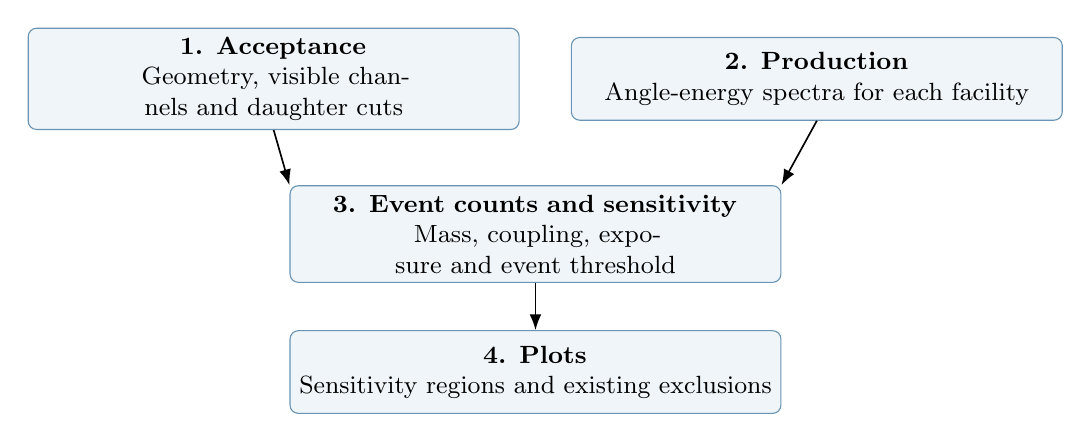
\begin{tikzpicture}[
  box/.style={draw=linkblue!65,fill=lightblue,rounded corners=3pt,align=center,
    text width=6.0cm,minimum height=1.05cm,font=\small},
  >={Latex[length=2mm]}]
 \node[box] (a) {\textbf{1. Acceptance}\\Geometry, visible channels and daughter cuts};
 \node[box,right=0.65cm of a] (b) {\textbf{2. Production}\\Angle-energy spectra for each facility};
 \node[box,below=0.7cm of a,xshift=3.325cm] (c)
  {\textbf{3. Event counts and sensitivity}\\Mass, coupling, exposure and event threshold};
 \node[box,below=0.6cm of c] (d)
  {\textbf{4. Plots}\\Sensitivity regions and existing exclusions};
 \draw[->,semithick] (a.south) -- (c.north west);
 \draw[->,semithick] (b.south) -- (c.north east);
 \draw[->,semithick] (c) -- (d);
\end{tikzpicture}
\end{center}

\subsection{Precision and physical assumptions}
Decay acceptance is estimated from sampled rest-frame decays, which are boosted, transported through the detector and subjected to the chosen cuts. The numerical integration uses the tabulated angle, energy and position dependence. Sampling statistics determine the precision of the acceptance estimate; the interpolation grids control how sharply varying features are resolved.

In the long-lifetime limit, $\lambda_z$ exceeds the detector dimensions and the exponential in Eq.~\eqref{eq:lifetime} varies little across the volume. The yield then depends approximately on the inverse proper lifetime, the inverse boost, the available path length and the efficiency for visible daughters. At larger couplings, decays upstream of the fiducial volume suppress the signal. This is why the same experiment can have both a lower and an upper sensitivity boundary.

The method and comparisons with experimental sensitivity estimates are presented in \arxiv{2305.13383}. Production and decay choices remain physical inputs to a prediction. The selected event threshold connects the expected count to the statistical analysis, including its assumptions about backgrounds.

\section{Installation and first calculation}\label{sec:start}
\subsection{Software and repository}
Use Mathematica 14.1 or later, \href{https://feyncalc.github.io/}{FeynCalc}, and a C/C++ compiler recognized by Mathematica. Wolfram's \href{https://reference.wolfram.com/language/CCompilerDriver/tutorial/SpecificCompilers.html}{compiler documentation} lists supported choices for each platform. The interactive workflow uses the notebook front end.

Download the complete repository, or clone it:
\begin{Code}
git clone https://github.com/maksymovchynnikov/SensCalc.git
\end{Code}
Keep its directory tree together. Main notebooks locate the model data and shared routines relative to their own directory. Files in cloud storage must be available locally before the calculation begins.

Open \code{0. Check for the needed soft.nb} and evaluate its two cells. The compiler query should identify a working installation, and FeynCalc should load. A direct compilation check is
\begin{Code}
cf = Compile[{{x, _Real}}, x*x, CompilationTarget -> "C"];
cf[2.]
\end{Code}
Successful evaluation returns \code{4.}.

The main calculation kernels compile during initialization. Native thread allocation follows Mathematica's settings. Runtime and memory use depend on the selected grids, decay multiplicity and sample sizes; increasing statistics is especially costly for rare accepted configurations.

\subsection{Example: a Higgs-mixed scalar at SHiP}
This example uses \code{Scalar} at \code{SHiP-ECN3}, with production through Higgs mixing. Its scan variable is the squared mixing angle defined in Section~\ref{sec:models}. At each stage, evaluate the top section labelled \textbf{Launch this section to run the notebook} using Shift+Enter.

\begin{enumerate}[itemsep=5pt]
\item \textbf{Acceptance.} Open \code{1. Acceptances.nb}. Choose \code{SHiP-ECN3}, the cuts in Section~\ref{sec:ship}, and \code{Scalar}. Select the visible decay channels, a decay description and the hadronization option. Review the geometry and export name. A distinct experiment name keeps a modified geometry or selection separate from other saved calculations.
\item \textbf{Production.} Open \code{2. LLP distribution.nb}. Choose \code{SPS}, then \code{Scalar}. For production through mixing, select the available channels ending in \code{mixing}, with proton bremsstrahlung if desired. Channels labelled \code{quartic} describe scalar-pair production. Choose the Monte Carlo sample size for the processes that require it.
\item \textbf{Sensitivity.} Open \code{3. Scalar sensitivity.nb}. Select the acceptance export, its decay description, and the production modes generated in step 2. Set $\Br(h\to SS)=0$ for this mixing-only example. Review the exposure and required signal count. The notebook exports event-count tables and the corresponding sensitivity regions.
\item \textbf{Plotting.} Open \code{4. Plots.nb}. Run the scalar chapter and select the saved results to compare. The figures are written under \code{plots/}.
\end{enumerate}

Notebook 2 allows several LLP models to be selected for one facility. It asks for the production channels of every selected model before starting generation. \textbf{All channels} refers to the model named in that dialog. The common sampling setting accepts an integer such as \code{10^6}.

The same sequence applies to \code{ALP-electroweak} and \code{ALP-fermion} at SHiP, \code{ALP-photon} at \code{FASER2-FPF}, or \code{Scalar} at MATHUSLA. For the last example, a nonzero choice such as $\Br(h\to SS)=0.01$ requires the corresponding pair-production spectra as well as the desired mixing contributions.

\subsection{Reusing results}
\begin{tabularx}{\linewidth}{@{}P{0.47\linewidth}Y@{}}
\toprule
Changed input & Required calculation \\
\midrule
Exposure or signal-event threshold & Rescaling or sensitivity calculation in notebook 3, then plotting. \\
Geometry, detectable species or cuts & Acceptance, event counts and sensitivity, then plotting. \\
Decay widths, branching fractions or matrix elements & Acceptance and all dependent results; regenerate decay samples when their physical model changes. \\
Mother spectra or production-channel mixture & LLP spectra and all dependent results. \\
Mass range & Extend the relevant physical inputs and grids before the dependent calculations. \\
Figure appearance & Plotting only. \\
\bottomrule
\end{tabularx}

Production spectra are reusable for experiments sharing the same facility inputs, including beam conditions and target material. After editing model or geometry definitions, initialize a fresh kernel so compiled functions incorporate those changes. A notebook edit by itself does not alter previously exported tables.

\section{Models and coupling conventions}\label{sec:models}
Model identifiers appear in dialogs, filenames and notebook definitions. The three pure-flavour heavy-neutral-lepton inputs are grouped under \code{HNL} in the interface. Inelastic models have additional identifiers for their fixed mass parameters.

\subsection{Heavy neutral leptons}
The models \code{HNL-mixing-e}, \code{HNL-mixing-mu} and \code{HNL-mixing-tau} contain a heavy neutral lepton $N$ mixed with the indicated neutrino flavour. Their charged-current interaction is
\begin{equation}
 \mathcal L\supset-\frac{g_2}{\sqrt{2}}\sum_{\alpha=e,\mu,\tau}
 U_\alpha W^-_\mu\,\bar\ell_\alpha\gamma^\mu P_LN+\hc,
\end{equation}
with the corresponding neutral current fixed by electroweak mixing. Here $g_2$ is the weak gauge coupling, $P_L$ projects onto left chirality, and $U_\alpha$ denotes mixing with flavour $\alpha$.

The sensitivity calculation combines the flavour inputs at fixed ratios of $|U_\alpha|^2$ and scans their total $U^2=\sum_\alpha|U_\alpha|^2$. The selected Dirac or Majorana nature affects decay rates and accessible final states. Production includes meson, lepton and electroweak-boson decays where the facility provides their spectra. The main phenomenological reference is \arxiv{1805.08567}.

\subsection{Higgs-mixed scalar}
The interactions of \code{Scalar} are defined by
\begin{equation}
 \mathcal L\supset\theta m_h^2hS+\frac{\alpha}{2}hS^2.
\end{equation}
The fields $h$ and $S$ denote the Higgs boson and the lighter scalar, $m_h$ is the Higgs mass, $\theta$ is a small mixing angle, and $\alpha$ is a trilinear coupling in GeV. The scan parameter is $\theta^2$; pair production is parameterized by $\Br(h\to SS)$.

Mixing produces \code{Scalar} through meson decays and proton bremsstrahlung, while the Higgs coupling creates pairs. Alternative hadronic decay descriptions change the widths into pions and kaons, and therefore the lifetime and visible branching fractions. See \arxiv{1904.10447} for production and \arxiv{2407.13587} for hadronic widths.

\subsection{Dark photon and baryon/lepton vector bosons}
The low-energy kinetic mixing of \code{DP} is
\begin{equation}
 \mathcal L\supset\frac{\epsilon}{2}V_{\mu\nu}F^{\mu\nu},
\end{equation}
where $V_{\mu\nu}$ and $F_{\mu\nu}$ are the dark-photon and electromagnetic field strengths. The sensitivity scan uses $\epsilon^2$. Meson decays, bremsstrahlung and Drell-Yan production are available according to the facility inputs. The treatment of hadronic production and event generation is discussed in \arxiv{2409.11096}; production through mixing during fragmentation is described in \arxiv{2504.06828}.

The baryon/lepton vector models use the interaction and scan variable
\begin{equation}
 \mathcal L\supset g_B V_\mu\left(J_B^\mu+
 \sum_{\alpha=e,\mu,\tau}x_\alpha J_{L_\alpha}^\mu\right),
 \qquad \alpha_B=\frac{g_B^2}{4\pi}.
\end{equation}
The currents $J_B^\mu$ and $J_{L_\alpha}^\mu$ count baryon number and individual lepton flavours. Their coefficients are
\begin{center}
\begin{tabular}{@{}lc@{}}
\toprule
Model & $(x_e,x_\mu,x_\tau)$ \\
\midrule
\code{B} & $(0,0,0)$ \\
\code{B-L} & $(-1,-1,-1)$ \\
\code{B-3Lmu} & $(0,-3,0)$ \\
\code{B-3Le-Lmu+Ltau} & $(-3,-1,1)$ \\
\code{B-Le-3Lmu+Ltau} & $(-1,-3,1)$ \\
\bottomrule
\end{tabular}
\end{center}
The \code{B} current is anomalous; its meson production depends on the assumptions about the ultraviolet theory. The relevant vector phenomenology is summarized in \arxiv{1801.04847}.

\subsection{Axion-like particles}
For an axion-like field $a$, define the dual field strength as $\widetilde X^{\mu\nu}=\tfrac12\epsilon^{\mu\nu\rho\sigma}X_{\rho\sigma}$. SensCalc uses the following interactions:
\begin{align}
 \code{ALP-photon}:\quad &\mathcal L\supset\frac{g_{a\gamma\gamma}}{4}aF_{\mu\nu}\widetilde F^{\mu\nu},\\
 \code{ALP-fermion}:\quad &\mathcal L\supset\frac{\partial_\mu a}{f_a}\sum_f\bar f\gamma^\mu\gamma_5f,\\
 \code{ALP-gluon}:\quad &\mathcal L\supset\frac{\alpha_s}{4\pi f_a}aG^A_{\mu\nu}\widetilde G^{A\mu\nu},\\
 \code{ALP-electroweak}:\quad &\mathcal L\supset\frac{\alpha_2g_W}{4\pi}aW^I_{\mu\nu}\widetilde W^{I\mu\nu}.
\end{align}
Here $f_a$ is an interaction scale in GeV; $\alpha_s$ and $\alpha_2$ are the strong and weak fine-structure constants, and $A$ and $I$ label gluon and weak gauge fields. The fermion and gluon interactions are defined at 1 TeV. Evolution to lower energies induces other couplings.

\begin{tabularx}{\linewidth}{@{}P{0.31\linewidth}P{0.26\linewidth}Y@{}}
\toprule
Model & Scan parameter & Main production mechanisms \\
\midrule
\code{ALP-photon} & $g_{a\gamma\gamma}$ in $\GeV^{-1}$ & Primary and cascade Primakov production, photon fusion, radiative meson decays. \\
\code{ALP-fermion} & $y=2v/f_a$, dimensionless & Heavy and light meson decays and hadronic production. \\
\code{ALP-gluon} & $f_a^{-1}$ in $\GeV^{-1}$ & Meson decays and hadronic production. \\
\code{ALP-electroweak} & $g_W$ in $\GeV^{-1}$ & $B$ and charged-kaon decays, primary and cascade Primakov production. \\
\bottomrule
\end{tabularx}

The electroweak vacuum expectation value is $v\simeq246\,\GeV$. For \code{ALP-fermion}, \textbf{Default} denotes the decay description based on \arxiv{2501.04525}; alternative descriptions are available in the model dialog. The selected branching fractions and lifetime must be used together.

Production of \code{ALP-fermion} in $B$ decays includes strange recoil states and $B\to\pi a$, combined with their relative branching fractions. At SPS, $K^\pm\to\pi^\pm a$ uses the spectrum of charged kaons decaying in flight and the normalization of 0.36 such kaon decays per incident proton from \arxiv{2004.07974}. The $K_S\to\pi^0a$ contribution is separate.

The hadronic ALP descriptions are discussed in \arxiv{2501.04525}. Photophilic production is described in \arxiv{1904.02091}, with electromagnetic cascades treated in \arxiv{2606.07743}. Mechanism availability depends on the photon, meson and scattering inputs for the chosen facility.

\subsubsection{Electroweak ALP lifetime, production and exclusions}
For \code{ALP-electroweak}, the induced diphoton coupling and decay width are
\begin{equation}
 g_{a\gamma\gamma}=\frac{\alpha_{\mathrm{em}}}{\pi}g_W,
 \qquad
 \Gamma_{\gamma\gamma}=\frac{\alpha_{\mathrm{em}}^2m_a^3g_W^2}{64\pi^3}.
\end{equation}
Here $m_a$ is the ALP mass and $\alpha_{\mathrm{em}}$ the electromagnetic fine-structure constant. The model sets $\Br(a\to\gamma\gamma)=1$, following the diphoton approximation of \arxiv{2609.19269}. The proper decay length is
\begin{equation}
 c\tau=\frac{1.973269804\times10^{-16}\;\GeV\,\mathrm{m}}{\Gamma_{\gamma\gamma}}.
\end{equation}
The lifetime table covers $0.001$ to $10\,\GeV$ at $g_W=1\,\GeV^{-1}$ and scales as $g_W^{-2}$. The acceptance grid covers $0.02$ to $5.12\,\GeV$. Production grids cover $0.02$ to $5.12\,\GeV$ for $B$ decays, $0.02$ to $0.354\,\GeV$ for charged-kaon decays, and $0.02$ to $4\,\GeV$ for Primakov production; individual recoil thresholds further restrict these ranges.

Relative rates into the exclusive strange recoil states in $B$ decays follow the Higgs-like scalar ratios, normalized to the electroweak-ALP $B\to Ka$ rate. The $B\to\pi a$ contribution uses the corresponding scalar ratio for the transition to a down quark. Primakov spectra use the photophilic kinematics with the diphoton coupling above; primary and cascade photons contribute separate spectra and probabilities.

\textbf{Acknowledgment of exclusion data.} The existing bounds are taken from the \href{https://github.com/KlingFelix/FORESEE/tree/main/Models/ALP-W}{ALP-W model in the FORESEE repository}, by Felix Kling and Sebastian Trojanowski. SensCalc combines the laboratory bounds into one ordered closed contour and keeps the astrophysical bound separately. FORESEE's convention $\mathcal L\supset-g_{aWW}aW\widetilde W/4$ is converted using $g_W=\pi|g_{aWW}|/\alpha_2$. Source references and the conversion are also documented alongside the exclusion files.

\subsection{Inelastic dark matter and other dark-sector states}
\paragraph{Dark-photon-mediated inelastic dark matter.}
The \code{Inelastic-DP-DM} family contains a light fermion $\chi$ and a heavier state $\chi'$, with the transition interaction
\begin{equation}
 \mathcal L\supset\frac{\epsilon}{2}V_{\mu\nu}F^{\mu\nu}
 +\sqrt{4\pi\alpha_D}\,V_\mu\bar\chi'\gamma^\mu\chi+\hc.
\end{equation}
The parameter $\alpha_D$ is the dark-sector fine-structure constant. A dark photon with $m_V>m_\chi+m_{\chi'}$ produces the two states through an on-shell decay. The heavier one subsequently decays through an off-shell mediator into $\chi$ and visible particles. Its boost and lifetime determine the displaced signal. SensCalc scans $\epsilon^2\alpha_D$ for the mass ratios of the selected model. See \arxiv{2012.08595} for the inelastic model and \arxiv{2409.11096} for the mediator production.

\paragraph{Electromagnetic transition dipole.}
The \code{Inelastic-dipole-DM} family uses
\begin{equation}
 \mathcal L\supset\frac{\mu}{2}F^{\mu\nu}\bar\chi_1\sigma_{\mu\nu}\chi_0+\hc,
\end{equation}
where $\chi_1$ is the heavier fermion, $\chi_0$ the lighter state, $\sigma_{\mu\nu}=i[\gamma_\mu,\gamma_\nu]/2$, and $\mu$ the dipole coupling in $\GeV^{-1}$. The visible decay contains a photon, $\chi_1\to\chi_0\gamma$. The chosen model fixes the mass splitting; the phenomenology is discussed in \arxiv{2301.05252}.

\paragraph{Dark hadrons.}
The \code{Dark-QCD-rho} model describes a dark vector meson $\rho_D$ whose visible decay is induced by a heavy vector mediator $Z'$. The latter couples to a dark current $J_D^\mu$ and mixes with the hypercharge field strength $B^{\mu\nu}$:
\begin{equation}
 \mathcal L\supset\frac{\kappa}{2\cos\theta_W}Z'_{\mu\nu}B^{\mu\nu}
 +e_D Z'_\mu J_D^\mu,
 \qquad \Lambda^{-2}=\frac{\kappa e_D e}{m_{Z'}^2}.
\end{equation}
Here $e_D$ and $e$ are the dark and electromagnetic gauge couplings, $\theta_W$ is the weak mixing angle, and $\Lambda$ is an effective interaction scale in GeV. The scan uses $\Lambda^2$ with $e_D=1$ and the fixed mediator parameters in the model definition. The decay descriptions follow \arxiv{2203.08824} and \arxiv{2311.17157}.

\paragraph{Millicharged particles.}
The \code{MCP} production calculation uses $\mathcal L\supset\epsilon eA_\mu\bar\chi\gamma^\mu\chi$, where $\chi$ has charge $\epsilon e$. Notebook 2 returns its flux. See \arxiv{2205.09137} for the production phenomenology.

\subsection{Mass coverage}
A sensitivity point requires overlapping production, acceptance, lifetime and branching-fraction inputs. Meson decays close at the mother mass minus the recoil masses; scattering and hadronized-decay tables have their own domains.

After initialization, \code{mLLPlist[model]} in notebook 1 and \code{MassList[model, productionMode, facility]} in notebook 2 give the available nodes. The sensitivity calculation uses the common mass interval. Section~\ref{sec:formats} shows how to inspect exported tables.

\section{Experiments and selection cuts}\label{sec:experiments}
\subsection{Facilities and geometry}
An experiment definition combines the beam facility, exposure, mother-particle yields, fiducial decay volume, detector planes and magnetic field. Representative choices are listed below; each notebook's dialog displays the setups and input spectra available for that calculation.

\begin{tabularx}{\linewidth}{@{}P{0.27\linewidth}Y@{}}
\toprule
Facility & Examples \\
\midrule
SPS & SHiP-ECN3, SHiP-ECN4, SHADOWS, HIKE-dump, NA62-dump, CHARM, BEBC. \\
Fermilab beam dump & DUNE near-detector configurations and DarkQuest. \\
Serpukhov & NuCal. \\
LHC & FASER, FASER2, FACET, PREFACE, MATHUSLA, CODEX-b, ANUBIS, SND and LHCb configurations. \\
Other facilities & FCC-hh configurations, SLAC-E137, ESS/SHiNESS and SuperKEKB/Belle II. \\
\bottomrule
\end{tabularx}

SHiP offers the two configurations \code{SHiP-ECN3} and \code{SHiP-ECN4}. The ANUBIS ceiling geometry has a dedicated \code{1. Acceptances. ANUBIS-ceiling.nb}; compatible shaft-module contributions can be combined at the event-count stage.

The beam defines the longitudinal axis. A ray emitted from the origin satisfies $x=z\tan\theta\cos\phi$ and $y=z\tan\theta\sin\phi$, with azimuth $\phi$. For an off-axis or annular volume, only part of the azimuthal range reaches the fiducial region. Daughter trajectories are projected onto the relevant detector planes, including charged-particle bending where a magnet is part of the setup. Electromagnetic-calorimeter availability determines which neutral final states are detectable.

\subsection{Meaning of the cuts}
The acceptance dialog controls individual energy and transverse-momentum thresholds, particle species, multiplicity, and pair requirements such as invariant mass, pair energy, separation and impact parameter. The impact parameter measures the distance from the production point to the backward projection of the pair's combined momentum.

For \textbf{\code{>=2}}, a qualifying pair must have zero total electric charge and satisfy the active daughter and pair cuts. Larger multiplicity choices require the corresponding number of detectable products. \textbf{All detectable} requires every visible daughter to pass its own geometry, energy and transverse-momentum cuts; pair cuts are disabled for that signature. A veto rejects forbidden species independently of whether they would be detected. The \code{Null} option denotes no veto.

Decay-channel selection enters both $\Br_{\mathrm{vis}}$ and the conditional efficiency in Eq.~\eqref{eq:yield}. Selecting all physically allowed modes does not guarantee that their daughters are detectable. Neutral, invisible and out-of-acceptance particles contribute according to the chosen signature.

\subsection{Preferred SHiP selection}\label{sec:ship}
For the two SHiP setups, the following starting selection follows \href{https://cds.cern.ch/record/2878604?ln=en}{\emph{BDF/SHiP at the ECN3 high-intensity beam facility}, CERN-SPSC-2023-033}.

\begin{tabularx}{\linewidth}{@{}P{0.32\linewidth}Y@{}}
\toprule
Setting & Choice \\
\midrule
Signature & \code{>=2} detectable particles. \\
Individual energy & Above $1\,\GeV$ for electrons, muons, charged hadrons, photons and neutral hadrons. \\
Impact parameter & Below $2.5\,\mathrm{m}$. \\
Decay channels & All allowed channels. \\
Other optional kinematic cuts & Disabled. \\
\bottomrule
\end{tabularx}

Enter these values in notebook 1: selecting the experiment loads its geometry, while the cut dialog determines the event selection. Each daughter used to satisfy the signature is subject to the energy threshold.

\subsection{NA62 in dump mode}
Appendix C.4 of \arxiv{2405.08081} gives a reference selection informed by discussions with collaboration members. It requires at least two charged decay products inside the detector acceptance, each with momentum above $1\,\GeV$. Muon pairs must be separated by at least $0.02\,\mathrm{m}$ at the first straw station; electron and hadron pairs must be separated by at least $0.20\,\mathrm{m}$ at the ECAL entrance.

For relativistic daughters, the individual energy cut $E>1\,\GeV$ is the practical approximation to the momentum requirement. The paper's example with an invisible daughter uses no numerical impact-parameter threshold.

The dialog exposes one charged-particle separation threshold. Although the transport routines distinguish muon and non-muon projection planes, the \code{NA62-dump} definition places both at the downstream detector plane. Reproducing the reference selection's two separation requirements exactly therefore requires species-dependent thresholds and the appropriate planes in the experiment definition. The energy approximation alone does not make the full selection identical to that study.

\section{Computing acceptance}\label{sec:acceptance}
\code{1. Acceptances.nb} builds $\epsilon_{\mathrm{az}}$ and $\epsilon_{\mathrm{dec}}$ on a grid in mass, polar angle, energy and decay position. It also exports the selected visible branching fraction, lifetime and experiment information needed for the yield integration.

\subsection{Decay descriptions and sampling}
The initialization loads model definitions, presents available decay descriptions and constructs compatible mass grids. A model with one description keeps that choice as its default. Selecting several descriptions produces separate acceptance results, each with its own branching fractions and lifetime.

Two-body decays use their rest-frame kinematics. Three-body channels sample the daughter energies according to the matrix-element weight, then generate orientations and boost the momenta into the laboratory. The sampling uses the magnitude of each weight; nonnumeric, nonfinite or zero-support distributions are rejected. The daughter ordering in the squared amplitude must match the channel definition. Generic four-body channels use the implemented phase-space treatment.

For hadronic final states, SensCalc can use precomputed \href{https://github.com/maksymovchynnikov/exHad}{exHad} samples at their tabulated masses, following the hadronization model of \arxiv{2609.16104}. The alternative treatment represents the decay through the implemented hadronic proxies. Unstable daughters are decayed according to the model routines before their visible products are tested against the detector requirements.

The total efficiency averages channel efficiencies with their physical branching fractions. A rare decay mode therefore contributes with its branching weight even when the Monte Carlo assigns it enough events to resolve its kinematics. A description with no support in the selected channels produces no acceptance table. If a table with the same name exists, the notebook identifies it before proceeding so it cannot be mistaken for the result of that selection.

\subsection{Geometry, transport and progress}
Azimuthal acceptance is evaluated over the allowed rays for each angle and longitudinal position. Compiled routines boost the sampled daughters, apply individual cuts, propagate charged particles through the field, and evaluate pair requirements. The resulting efficiency remains conditional on an allowed LLP decay vertex.

The progress display shows the model, experiment, current mass, completed points, elapsed time and an estimate of the remaining duration. It updates between mass points. A long interval without a display change can therefore correspond to the current mass calculation.

The settings controlling decay statistics and the mass, angle, energy and position grids are in the notebook's calculation sections. Larger samples improve statistical precision; denser tabulation resolves rapid dependence on these variables. These choices belong with the physical selection when comparing predictions.

\subsection{Saved acceptance}
The output has the form
\begin{Code}
Acceptances/<experiment>/
  Acceptance_<experiment>_for_<model>_decayDescription_<description>.m
\end{Code}
This file uses Wolfram MX binary format. Its seven elements contain the facility, calorimeter availability, numeric acceptance table, exposure and parent yields, visible branching fraction, description text and proper lifetime. Column definitions and an import example are given in Section~\ref{sec:formats}.

\section{Computing production spectra}\label{sec:production}
\code{2. LLP distribution.nb} calculates the normalized angle-energy distributions $f_i(\theta,E)$ for each mass. Its inputs are the selected facility's mother spectra, decay amplitudes, scattering descriptions and relative production rates.

\subsection{Selection and generation}
Choose a facility, select one or more LLPs, then choose the production channels separately for each. Generation begins after those choices are collected. Availability follows the mechanism definitions and the spectra present for that facility.

For meson and lepton decays, the calculation samples mother momenta, generates the decay in its rest frame and boosts the LLP. When several exclusive decays contribute to a common spectrum, their fractions determine the mixture. Both kinematics and relative rates depend on the LLP mass. The absolute number produced is incorporated in notebook 3.

Primakov production converts a photon into an ALP in the nuclear electromagnetic field. Primary photons and photons from an electromagnetic cascade have different spectra and normalizations. Their contributions are offered separately where the relevant inputs exist. Photon fusion, bremsstrahlung and Drell-Yan production use their corresponding scattering or pregenerated distributions.

Production involving neutral-meson mixing can use distributions from hadronic event generation, following \arxiv{2504.06828}. Such files are part of the required inputs. Generating external \href{https://pythia.org/}{Pythia} or \href{https://launchpad.net/mg5amcnlo}{MadGraph} samples is a separate calculation from the ordinary four-notebook sequence.

\subsection{Normalization and output}
The distribution density is defined with respect to $\dd\theta\,\dd E$ and normalized according to the facility's angular domain. Mother yields, branching fractions, scattering probabilities and LLP multiplicities enter the absolute production probability. Using a shape from one description with the rate of another changes the physical prediction.

Standard exports have the form
\begin{Code}
spectra/New physics particles spectra/<model>/
  DoubleDistr_<model>_<production>_<facility>.m
\end{Code}
They contain mass, polar angle, energy and probability density. All pure-flavour HNL cases use the \code{HNL/} directory. Bremsstrahlung exports can hold several named descriptions with their associated tables; probability files are stored under the model's phenomenology directory.

Sample size controls both runtime and memory. Processes drawing large mother and decay samples can require substantial memory, especially when several generations are retained simultaneously. Facility runs can be performed separately while preserving the same physical grids and channel choices.

\section{Event counts, sensitivity and plots}\label{sec:sensitivity}
\subsection{From production probabilities to a yield}
The model-specific \code{3. ... sensitivity.nb} imports acceptance and production tables, then evaluates Eq.~\eqref{eq:yield}. Select the experiment export, decay description, production modes, exposure and model parameters. Each included mode needs both its distribution and the production probability with the same coupling convention.

The default integration uses numerical sums over the tabulated variables, with interpolation as defined by the calculation. Some model notebooks also expose direct numerical integration for comparison. Coupling dependence enters the production normalization, the visible branching fraction when relevant, and the boosted lifetime. Strong changes near thresholds or short lifetimes can require finer grids.

The event tables separate production contributions, allowing different combinations to be compared without regenerating their kinematics. A contour is the boundary at a chosen count $N_{\min}$. Its statistical interpretation follows the signal threshold selected for the analysis; background estimates and a confidence-level construction are needed to assign that interpretation.

For \code{Scalar}, mixing and Higgs-pair contributions are combined at the selected $\Br(h\to SS)$. For \code{HNL}, the normalization is tied to the chosen flavour fractions and Dirac or Majorana nature. ANUBIS-shaft module tables can be added when their grids, exposure and decay description agree.

\subsection{Uncertainty regions}
Alternative production and decay descriptions quantify the dependence on physical inputs. A contribution without uncertainty variants remains part of every total in which it was selected. Scalar mixing and pair production use a common decay description when a scenario is combined, preserving their correlation through the lifetime and visible branching fractions.

For \code{ALP-fermion} and \code{ALP-gluon}, disconnected mass intervals are calculated separately and can run in parallel. Their contours retain the requested plotting resolution. The exported regions remain distinct ordered boundaries, so a gap in mass support is preserved in the figure.

Uncertainty regions describe the variations explicitly included in the chosen inputs. Sampling fluctuations, interpolation resolution and unvaried physics assumptions are separate sources of uncertainty.

\subsection{Saved results and plotting}
Event counts are written under \code{Tabulated Nevents/<model>/<experiment>/}. Sensitivity and uncertainty contours go to \code{Sensitivity domains/<model>/<experiment>/}. The adjacent metadata file records channels, descriptions, exposure, threshold and model-specific parameters. Reusing an existing output filename replaces that saved result; distinct experiment export names keep different configurations separate.

In \code{4. Plots.nb}, select the model chapter and the sensitivity files to compare. Existing exclusions are read from \code{contours/<model>/}; they use the coupling conventions in Section~\ref{sec:models}. Figures are saved under \code{plots/}. The diagnostic plots produced by model notebooks are stored in \code{plots/Production-plots/}.

HNL figures can contain different mixing patterns or particle natures. All selected curves are plotted; when their configurations differ, the shared title is ``HNLs'' and exclusion overlays are omitted. A common configuration enables its matching bounds and detailed title.

\section{Generating weighted decay events}\label{sec:events}
\code{EventCalc.nb} samples LLP momenta, decay vertices and daughter momenta from the production distributions. Its method accompanies \arxiv{2409.11096}. The generated events carry weights for the expected decay yield and can be used in subsequent detector studies.

\subsection{Running the generator}
Prepare the required spectra with notebook 2. Launch EventCalc and select the experiment, model, production modes and decay channels. Its model dialog offers \code{HNL}, \code{Scalar}, \code{DP}, \code{ALP-photon} and \code{ALP-fermion}.

After initialization, use
\begin{Code}
{expectedEvents, llpInfo, daughters} =
  NeventsBlock[mass, coupling1, coupling2, numberToSample];
\end{Code}
The model defines the coupling arguments; a second parameter is relevant when production has an independent interaction, as for a scalar pair. The examples in the initialized notebook specify these choices. The requested mass needs both production and decay data.

The underlying decay routine exposes the hadronization and secondary-decay choices:
\begin{Code}
SimulateFullEvent[mass, coupling1, coupling2, numberToSample,
  HadronizationOption, DecayUnstable]
\end{Code}
The final two arguments are the strings \code{"True"} or \code{"False"}. They select hadronized samples and decays of unstable daughters, respectively.

\subsection{Event weights}
The LLP table has one row for each generated decay. In that row, let $P_j$ be the probability of decay along the sampled ray and $w_j$ the azimuthal sampling weight. The returned yield is
\begin{equation}\label{eq:events}
 N_{\mathrm{events}}=N_{\mathrm{prod}}A\frac1n\sum_{j=1}^{n}P_jw_j,
\end{equation}
where $n$ is the sample size, $N_{\mathrm{prod}}$ the total production normalization and $A$ the fraction in the sampled angle-energy domain. These factors are stored with the event. Histograms of decay positions or daughter kinematics use the same weights $P_jw_j$.

For a ray at angles $(\theta,\phi)$, denote the length of its allowed interval in longitudinal coordinate by $L(\theta,\phi)$. The sampler chooses rays in proportion to that length. The compensating factor is
\begin{equation}
 w_j=\frac{I(\theta)}{L(\theta,\phi)},\qquad
 I(\theta)=\int\dd z\,\epsilon_{\mathrm{az}}(\theta,z).
\end{equation}
This factor can exceed unity and contributes to both the yield and the distributions. Its role is particularly relevant for off-axis geometries.

For \code{Scalar}, let $R_i$ be the production rate of component $i$ and $A_i$ its fraction in the sampled domain. Its sampling probability is $R_iA_i/\sum_k R_kA_k$, and the overall domain fraction is $A=\sum_i R_iA_i/\sum_i R_i$. This includes the different angular and energy populations of mixing and pair production.

\subsection{Event output}
Each call to \code{NeventsBlock} creates a directory of the form
\begin{Code}
Sampled Nevents/<experiment>/<model>/run-<id>/
\end{Code}
It contains the LLP information, daughter momenta and \code{metadata.json}. Keep them together: they specify the model parameters, channels, sample size and units needed to interpret Eq.~\eqref{eq:events}. The numeric tables use MX format. Daughter and LLP rows correspond event by event, and detector propagation and selection can be applied to the returned particles.

\section{Data formats and extensions}\label{sec:formats}
\subsection{Directory map}
All paths below are relative to the SensCalc root.

\begin{tabularx}{\linewidth}{@{}P{0.46\linewidth}Y@{}}
\toprule
Directory & Contents \\
\midrule
\code{codes/} & Shared routines and experiment definitions. \\
\code{phenomenology/<model>/} & Lifetimes, branching fractions, amplitudes and production probabilities. \\
\code{spectra/SM particles/} & Mother-particle spectra. \\
\code{spectra/}\newline\code{New physics particles spectra/} & LLP angle-energy distributions. \\
\code{simulated phase space/} & Rest-frame hadronized decay samples. \\
\code{Acceptances/} & Acceptance tables and experiment data. \\
\code{Tabulated Nevents/} & Counts as a function of mass and coupling. \\
\code{Sensitivity domains/} & Sensitivity contours and uncertainty regions. \\
\code{contours/} & Existing exclusions. \\
\code{Sampled Nevents/} & Weighted EventCalc samples. \\
\code{plots/} & Exported figures. \\
\bottomrule
\end{tabularx}

Several files with extension \code{.m} contain Wolfram MX binary data. Read them with the format used by the producing notebook; the filename extension alone does not identify the contents.

\subsection{Mother spectra, acceptance and production tables}
A mother spectrum named \code{DoubleDistr_<facility>_<mother>.txt} contains three columns: polar angle in radians, energy in GeV, and probability density with respect to $\dd\theta\,\dd E$. Its absolute yield enters separately through the experiment data.

An acceptance export is read with \code{Import[path, "MX"]} and has seven elements:
\begin{center}
\begin{tabular}{@{}cP{0.80\linewidth}@{}}
\toprule
Element & Meaning \\
\midrule
1 & Facility identifier. \\
2 & Electromagnetic-calorimeter availability. \\
3 & Numeric acceptance table. \\
4 & Exposure and parent-particle production data. \\
5 & Branching fraction of the selected decay modes, as a function of mass. \\
6 & Explanation of the decay description. \\
7 & Proper decay length in metres, as a function of mass and coupling. \\
\bottomrule
\end{tabular}
\end{center}
Each row of the acceptance table contains
\begin{Code}
mass_GeV   theta_rad   energy_GeV   z_m   epsilon_az   epsilon_dec
\end{Code}
A standard LLP production table has four columns:
\begin{Code}
mass_GeV   theta_rad   energy_GeV   probability_density
\end{Code}
For a standard spectrum and an acceptance export, their mass domains can be inspected with
\begin{Code}
spectrum = Import[spectrumPath, "MX"];
acceptance = Import[acceptancePath, "MX"];
{
  "production masses" -> MinMax[spectrum[[All, 1]]],
  "acceptance masses" -> MinMax[acceptance[[3, All, 1]]]
}
\end{Code}
Set the two path variables to actual filenames. For an export with named production descriptions, select one distribution table before applying this example. Replacing \code{MinMax} by \code{DeleteDuplicates} returns the tabulated mass nodes.

\subsection{Counts, contours and decay samples}
Event-count text tables contain mass in GeV, the model's scan parameter and expected events. Sensitivity files begin with \code{Sensitivity_} and include the chosen production modes, uncertainty settings, decay description and ordered regions. MX exports preserve Wolfram expressions; JSON exports use named fields. Disconnected regions are stored as separate lists.

Closed exclusion contours follow consecutive boundary vertices and repeat the first point at the end. Sorting their coordinates by mass would generally destroy that ordering. Their physical assumptions and sources belong with the model's exclusion data.

Rest-frame decay samples and EventCalc daughters use eight entries per particle:
\begin{Code}
px   py   pz   energy   mass   PDG_identifier   electric_charge   stability
\end{Code}
The first five entries are in GeV, electric charge is in proton-charge units, and stability is \code{1.} for stable or metastable particles and \code{0.} for unstable ones. PDG identifiers are numeric; for example a photon has \code{22.}. Events with fewer daughters are padded on the right with \code{-999.} to form a rectangular array. Padding is missing data.

The EventCalc LLP information has the following columns:
\begin{center}
\begin{tabular}{@{}cP{0.78\linewidth}@{}}
\toprule
Columns & Quantity \\
\midrule
1 to 3 & LLP momentum components in GeV. \\
4, 5 & Energy and mass in GeV. \\
6, 7 & Cosine of the polar angle and momentum divided by mass. \\
8 & Decay probability $P_j$ along the allowed ray. \\
9 to 11 & Decay position $x,y,z$ in metres. \\
12 & Azimuthal weight $w_j$. \\
13 & Total production normalization $N_{\mathrm{prod}}$. \\
14 & Angle-energy fraction $A$. \\
\bottomrule
\end{tabular}
\end{center}

\subsection{Adding a model or production channel}
Use the implemented model closest in spin, decay topology and production mechanism as a starting point. Common routines generate decays, boost particles and apply the geometry; model definitions supply the physical quantities they need.

The decay definition in \code{codes/Acceptances/<model>.nb} includes the model description, coupling symbol, decay descriptions, proper lifetime, branching fractions and daughter identities. The lifetime function returns metres; its name contains the Greek letter $\tau$, written as \code{\[Tau]} in Wolfram input. The channel functions give the branching fractions and daughter identities:
\begin{Code}
c\[Tau]LLP[model, description, mass, coupling]
ListBrRatios[model, mass, process, description]
ListDecayProducts[model, process]
\end{Code}
The daughter list has four entries, with unused positions set to the string \code{"Null"}. Three-body squared amplitudes use the parent mass and the rest-frame energies of daughters 1 and 3. Their ordering must agree with the decay list. A common overall factor cancels when sampling a normalized shape, while relative terms and interference determine the distribution.

Register the acceptance mass grid and model launch section in notebook 1. Branching fractions, lifetime, thresholds and available decay samples must describe the same physical model across that domain.

Production definitions under \code{codes/LLP distribution/} use
\begin{Code}
ProcessesListAll[model]
ProductionType[model, process]
ReactionProductsList[model, process]
Msquared3Body[model, process, mass, E1, E3]
\end{Code}
The reaction list places the mother first and the LLP last. Relative branching fractions set the mixture when several processes contribute to one spectrum. Update the facility availability, mass grids and production sections in notebook 2; the latter follow the naming convention \code{<model>_<production>}. Preserve the existing notebook cell groups and tags used by the launch routines.

In the sensitivity notebook, \code{PmotherToLLP} must use the same production normalization and coupling convention as the spectra. Add a plotting chapter and any comparison bounds with their references. Sub-notebooks loaded from the code directories are Mathematica \code{.nb} files; generated plots belong under \code{plots/}.

\subsection{Defining an experiment and resolving input errors}
Experiment definitions reside in \code{codes/experiments.nb}. They specify exposure and parent yields, the decay volume, detector planes, detectable particles, magnetic field and beam geometry. Copying the closest physical setup provides the existing conventions. A changed decay volume or daughter selection requires regenerating acceptance before the sensitivity is recomputed.

When evaluation stops, start from its first reported error. An import failure identifies the missing input or incomplete local download. A missing production probability means that an available spectrum lacks the matching absolute normalization for that model and facility. Interpolation warnings can indicate a mass outside the common input domain. A vanishing yield may reflect a closed channel, an excluded decay mode, or zero acceptance.

The repository's Markdown guides cover the same tasks in a form convenient for browsing. The PDF and online documentation describe the current calculation; physical results also depend on the inputs and settings saved with each run.

\section{References and acknowledgments}\label{sec:references}
Please cite the SensCalc method and the works relevant to the physical inputs used in a calculation.

\begin{enumerate}[label={[\arabic*]},itemsep=4pt]
\item M.~Ovchynnikov, J.-L.~Tastet, O.~Mikulenko and K.~Bondarenko, \emph{Sensitivities to feebly interacting particles: public and unified calculations}, Phys.~Rev.~D \textbf{108}, 075028 (2023), \arxiv{2305.13383}.
\item Y.~Kyselov and M.~Ovchynnikov, \emph{Searches for long-lived dark photons at proton accelerator experiments}, Phys.~Rev.~D \textbf{111}, 015030 (2025), \arxiv{2409.11096}.
\item Y.~Kyselov, S.~Mrenna and M.~Ovchynnikov, \emph{New physics particles mixing with mesons: production in the fragmentation chain}, Phys.~Rev.~D \textbf{112}, 055033 (2025), \arxiv{2504.06828}.
\item M.~Climescu, M.~F.~Mikkelsen and M.~Ovchynnikov, \emph{SHiP as a (post-)discovery machine: identifying the diphoton signals' origin}, \arxiv{2609.19269}.
\item M.~Climescu, Y.~Kyselov and M.~Ovchynnikov, \emph{Detector performance at SHiP for cascade-produced long-lived particles}, Phys.~Rev.~D \textbf{114}, 056016 (2026), \arxiv{2606.07743}.
\item M.~Ovchynnikov and A.~Zaporozhchenko, \emph{Advancing the phenomenology of GeV-scale axion-like particles}, \arxiv{2501.04525}.
\item G.~Dalla Valle Garcia, F.~Kahlhoefer, M.~Ovchynnikov and T.~Schwetz, \emph{Not-so-inelastic Dark Matter}, \arxiv{2405.08081}.
\item V.~Kryshtal and M.~Ovchynnikov, \emph{Rethinking search signatures: Hadronic decays of GeV-scale feebly coupled particles}, \arxiv{2609.16104}.
\end{enumerate}

References for other model-specific ingredients accompany their definitions in Section~\ref{sec:models}. The \code{ALP-electroweak} exclusion data are credited there to FORESEE, with a direct link to its ALP-W model and the convention used for conversion.

SensCalc is distributed under the BSD 3-Clause License included in the repository. Questions and reproducible problems can be submitted through \href{https://github.com/maksymovchynnikov/SensCalc/issues}{GitHub issues} or sent to \href{mailto:o.maxim@gmail.com}{o.maxim@gmail.com}.

\end{document}
